\chapter[Resultados Parciais]{Resultados Parciais}
\label{cha:resultados-parciais}

Foi utilizado um \emph{script bash} pra executar o programa e calcular o tempo de cada execução que, juntamente com a saída do programa de estados, permite estimar o tempo de execução para o cálculo dos estados.

\section{Tempo de Execução}

Dado $d\!\in\![2,9]$ discos e $\ p\!\in\![2,5]$ peões, a quantidade distintas de estados [$B$] e o tempo (em segundos) do cálculo está representado nas Tabelas \ref{tab:quantidade-de-estados-e-tempo-com-p-2}, \ref{tab:quantidade-de-estados-e-tempo-com-p-3}, \ref{tab:quantidade-de-estados-e-tempo-com-p-4} e \ref{tab:quantidade-de-estados-e-tempo-com-p-5}. Além das tabelas, um gráfico também foi desenhado com as informações (Figura \ref{fig:crescimento-de-estados-de-acordo-com-numero-de-peoes-e-discos}) de crescimento da quantidade de estados de acordo com o número de peões e discos. Analisando as tabelas, o número de estados e, consequentemente, o tempo para calcular todos os estados, cresce rapidamente. Com o auxílio do gráfico, percebe-se que o crescimento é exponencial.

\begin{table}[ht]
\centering
\begin{tabular}{|c|c|c|c|}
\hline
\emph{p} & \emph{d} & [\emph{B}] & Seg\tabularnewline
\hline
\hline
2 & 2 & 27 & 0\tabularnewline
\hline
2 & 3 & 102 & 0\tabularnewline
\hline
2 & 4 & 361 & 0\tabularnewline
\hline
2 & 5 & 1251 & 0\tabularnewline
\hline
2 & 6 & 4296 & 0\tabularnewline
\hline
2 & 7 & 14746 & 1\tabularnewline
\hline
2 & 8 & 50746 & 3\tabularnewline
\hline
2 & 9 & 175230 & 19\tabularnewline
\hline
\end{tabular}
\caption{Quantidade de Estados e Tempo com P = 2}
\label{tab:quantidade-de-estados-e-tempo-com-p-2}
\end{table}

\begin{table}[ht]
\centering
\begin{tabular}{|c|c|c|c|}
\hline
\emph{p} & \emph{d} & [\emph{B}] & Seg\tabularnewline
\hline
\hline
3 & 2 & 150 & 0\tabularnewline
\hline
3 & 3 & 1219 & 1\tabularnewline
\hline
3 & 4 & 9082 & 1\tabularnewline
\hline
3 & 5 & 65195 & 19\tabularnewline
\hline
3 & 6 & 457855 & 653\tabularnewline
\hline
3 & 7 & 3173596 & 19929\tabularnewline
\hline
\end{tabular}
\caption{Quantidade de Estados e Tempo com P = 3}
\label{tab:quantidade-de-estados-e-tempo-com-p-3}
\end{table}

\begin{table}[ht]
\centering
\begin{tabular}{|c|c|c|c|}
\hline
\emph{p} & \emph{d} & [\emph{B}] & Seg\tabularnewline
\hline
\hline
4 & 2 & 825 & 0\tabularnewline
\hline
4 & 3 & 14907 & 2\tabularnewline
\hline
4 & 4 & 243200 & 462\tabularnewline
\hline
\end{tabular}
\caption{Quantidade de Estados e Tempo com P = 4}
\label{tab:quantidade-de-estados-e-tempo-com-p-4}
\end{table}

\begin{table}[ht]
\centering
\begin{tabular}{|c|c|c|c|}
\hline
\emph{p} & \emph{d} & [\emph{B}] & Seg\tabularnewline
\hline
\hline
5 & 2 & 4513 & 0\tabularnewline
\hline
5 & 3 & 178898 & 505\tabularnewline
\hline
5 & 4 & 6303528 & 526949\tabularnewline
\hline
\end{tabular}
\caption{Quantidade de Estados e Tempo com P = 5}
\label{tab:quantidade-de-estados-e-tempo-com-p-5}
\end{table}

\begin{figure}[ht]
\centering
	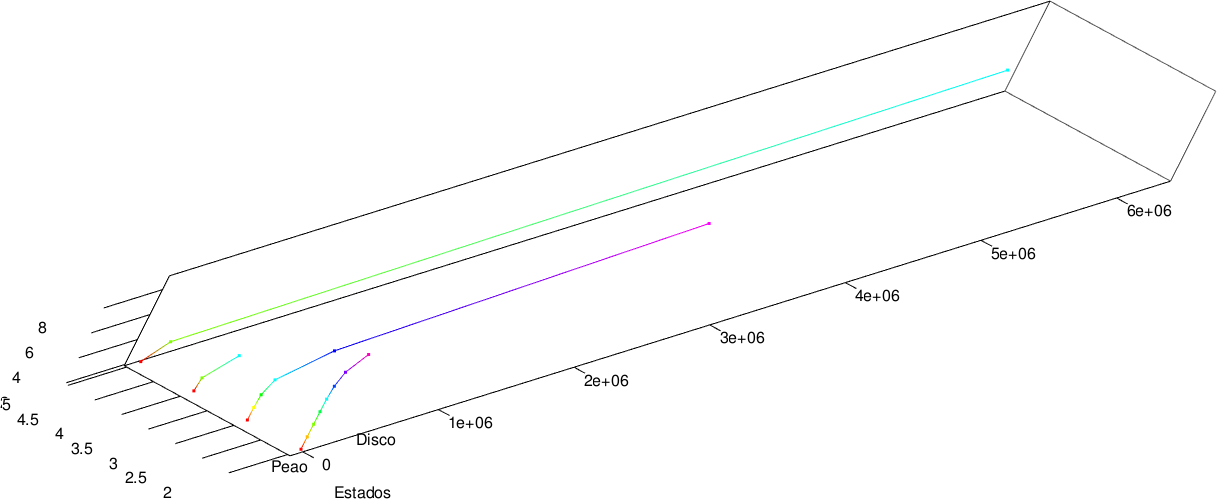
\includegraphics[keepaspectratio=true,scale=0.35]{figuras/graph_state.png}
\caption{Crescimento de estados de acordo com número de \emph{Peões} e \emph{Discos}}
\label{fig:crescimento-de-estados-de-acordo-com-numero-de-peoes-e-discos}
\end{figure}
